\begin{figure}
	\centering
	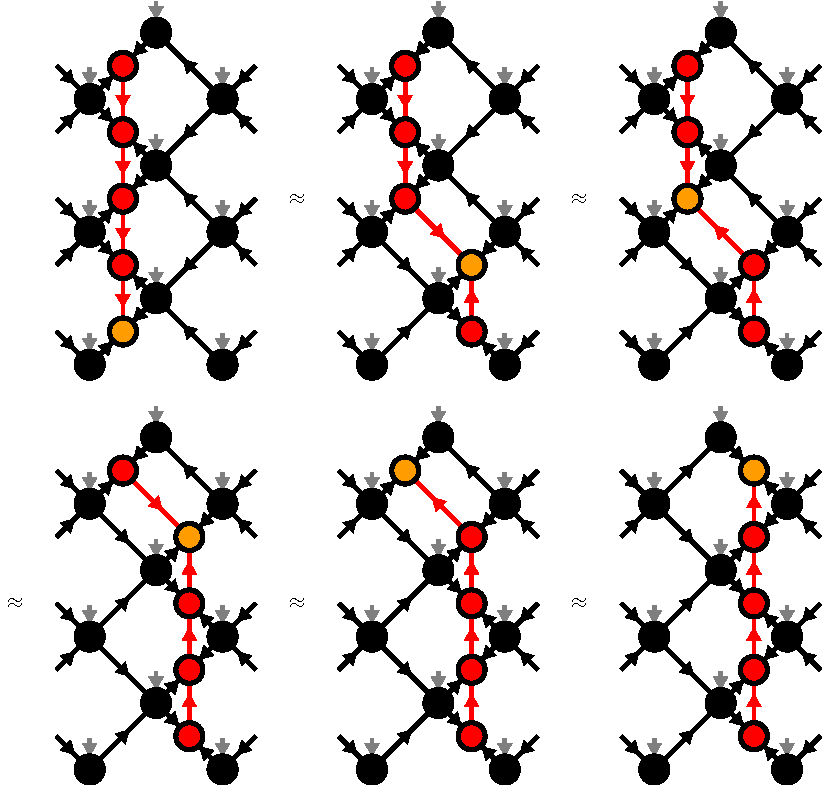
\includegraphics[scale=1]{figures/tikz/disoTPS/shifting_ortho_surface/shifting_ortho_surface.pdf}
	\caption{Two YB-moves are used to shift the orthogonality hypersurface one column to the right. In the last step, the orthogonality center can be moved across the $T$-tensor by contracting the two tensors and performing a truncated SVD.}
	\label{fig:disoTPS_moving_ortho_surface}
\end{figure}
Most algorithms implemented on disoTPS require an efficient procedure for moving the orthogonality surface, where the error introduced by this procedure should be as small as possible. For isoTPS, the current best procedure is given by the Moses Move, followed by an optional variational optimization. \par
In analogy to the MM we look for a procedure to iteratively shift the orthogonality surface through one column of $T$-tensors as shown in figure \figref{fig:disoTPS_moving_ortho_surface}. A single iteration of this process is shown in figure \figref{fig:disoTPS_YB_move_closeup}. The two tensors $W_1$ and $W_2$, which are part of the orthogonality hypersurface, are "pulled through" the site tensor $T$, resulting in the updated tensors $T^\prime$, $W_1^\prime$ and $W_2^\prime$. To keep the isometric structure of the network, $T^\prime$ and $W_1^\prime$ must be isometries, while $W_2^\prime$ must be a tensor of norm one (the new orthogonality center). Due to the visual similarity to the Yang-Baxter equation we call this procedure the \textit{Yang-Baxter} (YB) move. \par
We denote the state represented by the disoTPS before the YB move by $\left|\Psi\right\rangle = \left|\Psi\left(W_1, W_2, T\right)\right\rangle$ and the state after the YB move by $\left|\Psi^\prime\right\rangle = \left|\Psi^\prime\left(W_1^\prime, W_2^\prime, T^\prime\right)\right\rangle$. One can think of the YB move as an optimization problem
\begin{equation}
	\label{eq:disoTPS_YB_move_standard}
	\left(T^\prime_\text{opt},W_{1,\text{opt}}^\prime,W_{2,\text{opt}}^\prime\right) = \underset{T^\prime,W_1^\prime,W_2^\prime}{\argmin}\left\lVert \left|\Psi\right\rangle - \left|\Psi^\prime\right\rangle\right\rVert_\text{F}
\end{equation}
under the constraints
\begin{equation}
	\label{eq:disoTPS_YB_move_constraints}
	T^{\prime\dagger}T^\prime = \id, \quad W_1^{\prime\dagger}W_1^\prime = \id, \quad \left\lVert W_2^\prime \right\rVert_\text{F} = 1.
\end{equation}
One can rewrite the error of the YB move as
\begin{equation}
	\label{eq:disoTPS_YB_move_rewritten_error}
	\begin{split}
		\left\lVert \left|\Psi\right\rangle - \left|\Psi^\prime\right\rangle \right\rVert_\text{F} =& \sqrt{\left\langle\Psi\middle|\Psi\right\rangle + \left\langle\Psi^\prime\middle|\Psi^\prime\right\rangle - 2\Re\left\langle\Psi\middle|\Psi^\prime\right\rangle} \\
		=& \sqrt{2 - 2\Re\left\langle\Psi\middle|\Psi^\prime\right\rangle},
	\end{split}
\end{equation}
where in the second step we used the fact that the wave function is normalized to one, $\left\langle\Psi\middle|\Psi\right\rangle = \left\langle\Psi^\prime\middle|\Psi^\prime\right\rangle = 1$. It follows that the optimization problem of minimizing the error becomes the problem of maximizing the overlap
\begin{equation}
	\label{eq:disoTPS_YB_move_alternative_formulation}
	\left(T^\prime_\text{opt},W_{1,\text{opt}}^\prime,W_{2,\text{opt}}^\prime\right) = \underset{T^\prime,W_1^\prime,W_2^\prime}{\text{argmax}}\Re\left\langle\Psi\middle|\Psi^\prime\right\rangle
\end{equation}
under the constraints \eqref{eq:disoTPS_YB_move_constraints}. Because the only tensors that are changed by the YB move are $W_1$, $W_2$ and $T$ and the three tensors make up a subregion of the full network with only incoming arrows, we can use the isometry condition and the computation of the overlap $\langle\Psi|\Psi^\prime\rangle$ reduces to a contraction of only six tensors as shown in figure \figref{fig:YB_move_iterate_polar_overlap}.\par
\begin{figure}
	\centering
	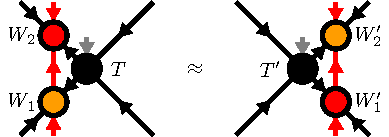
\includegraphics[scale=1]{figures/tikz/disoTPS/yang_baxter_move/yang_baxter_move.pdf}
	\caption{The Yang-Baxter (YB) move is the procedure of "pulling" two auxillary tensors $W_1$ and $W_2$ through a site tensor $T$.}
	\label{fig:disoTPS_YB_move_closeup}
\end{figure}
In the following, we present two explicit algorithms for performing the YB move. The first algorithm (see section \ref{sec:YB_move_iterative_local_optimization}) is an variational optimization method with iterative local updates. The second algorithm (see section \ref{sec:YB_move_svd_disentangle}) is a tripartite decomposition with disentangling similar to the tripartite decomposition used in the MM. In section \ref{sec:YB_move_comparison} we will compare the two algorithms.

\subsection{variational optimization with local updates}
\label{sec:YB_move_iterative_local_optimization}
To solve the constrained optimization problem \eqref{eq:YB_isoTPS_YB_move_alternative_formulation} we proceed by maximizing the overlap while only varying the parameters of one of the three tensors $T^\prime$, $W_1^\prime$ or $W_2^\prime$, treating all other tensors as constant. For example, let us keep $W_1^\prime$ and $W_2^\prime$ fixed and optimize $T^\prime$. We first contract all tensors except $T^\prime$ into an environment $E$ as shown in Figure \figref{fig:YB_move_iterate_polar_optimize_T}. We can then write the optimization problem as
\begin{equation}
	T^\prime_\text{opt} = \underset{T^{\prime\dagger}T = \id}{\argmax} \Re\braket{\Psi,\Psi^\prime} = \underset{T^{\prime\dagger}T = \id}{\argmax}\Re\left\langle E, T^\prime\right\rangle_\text{F} = \underset{T^{\prime\dagger}T = \id}{\argmax}\Re\Tr\left(T^{\prime\dagger}E\right).
\end{equation}
This problem is known as the \textit{orthogonal Procrustes problem} and permits the closed form solution $T^\prime_\text{opt} = UV^\dagger$, where $U$ and $V$ are computed using the SVD $E = USV^\dagger$. For the derivation of this solution see Appendix \ref{app:optimization_problems_for_isometric_tensor_networks}. The tensors $W_1^\prime$ and $W_2^\prime$ can be optimized similarly. The full algorithm is then performed by sweeping over the three tensors, optimizing them iteratively until convergence. Tensor diagrams for the algorithm are shown in Figure \figref{fig:YB_move_iterate_polar}. We discuss one iteration of the algorithm in more detail:
\begin{enumerate}
	\item Contract all tensors except $T^\prime$ into an environment $E$ and perform an SVD $E = USV$. The tensor $T^\prime$ is then updated as $T^\prime\leftarrow UV^\dagger$. See Figure \figref{fig:YB_move_iterate_polar_optimize_T}.
	\item Contract all tensors except $W_1^\prime$ into an environment $E$ and perform an SVD $E = USV$. The tensor $W_1^\prime$ is then updated as $W_1^\prime\leftarrow UV^\dagger$. See Figure \figref{fig:YB_move_iterate_polar_optimize_W1}.
	\item Contract all tensors except $W_2^\prime$ into an environment $E$. The tensor $W_1^\prime$ is then updated as $W_1^\prime\leftarrow E/\left\lVert E\right\rVert$. See Figure \figref{fig:YB_move_iterate_polar_optimize_W2}.
\end{enumerate}
These three steps are repeated until a termination criterion is met, for example until the decrease in error after one iteration is smaller than a given threshold or if a given maximum number of iterations $N_\text{iter}$ is exceeded. A similar algorithm was also used by Evenbly and Vidal in the context of the multi-scale entanglement renormalization ansatz
(MERA) \cite{cite:algorithms_for_entanglement_renormalization, cite:algorithms_for_entanglement_renormalization_boundaries_impurities_interfaces}. Note that in step three of the algorithm, a norm constraint is enforced instead of an isometry constraint, in which case the closed form solution takes a different shape. We also derive this solution in Appendix \ref{app:optimization_problems_for_isometric_tensor_networks}.\par
\begin{figure}
	\centering
	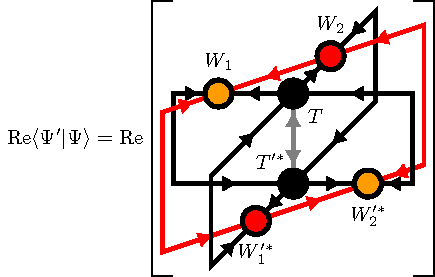
\includegraphics[scale=1]{figures/tikz/YB_isoTPS/yang_baxter_move_iterative/yang_baxter_move_iterative_a.pdf}
	\caption{The cost function of the optimization problem \eqref{eq:YB_isoTPS_YB_move_alternative_formulation} can be computed as a contraction of only six tensors.}
	\label{fig:YB_move_iterate_polar_overlap}
\end{figure}
\begin{figure}
	\centering
	\begin{subfigure}[c]{0.85\textwidth}
		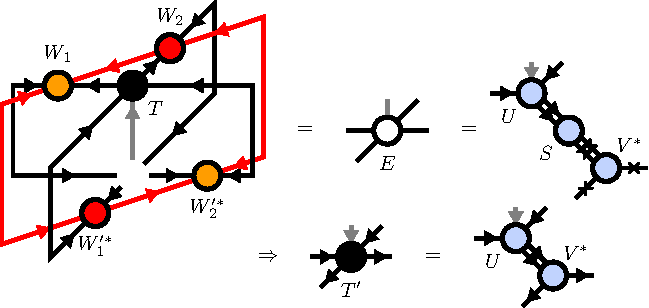
\includegraphics[scale=1]{figures/tikz/YB_isoTPS/yang_baxter_move_iterative/yang_baxter_move_iterative_b.pdf}
		\caption{}\label{fig:YB_move_iterate_polar_optimize_T}
	\end{subfigure}
	\begin{subfigure}[c]{0.85\textwidth}
		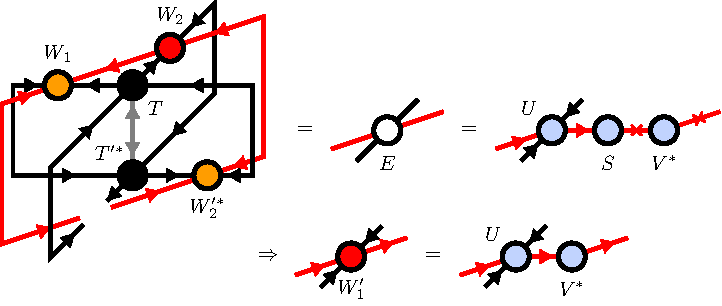
\includegraphics[scale=1]{figures/tikz/YB_isoTPS/yang_baxter_move_iterative/yang_baxter_move_iterative_c.pdf}
		\caption{}\label{fig:YB_move_iterate_polar_optimize_W1}
	\end{subfigure}
	\begin{subfigure}[c]{0.85\textwidth}
		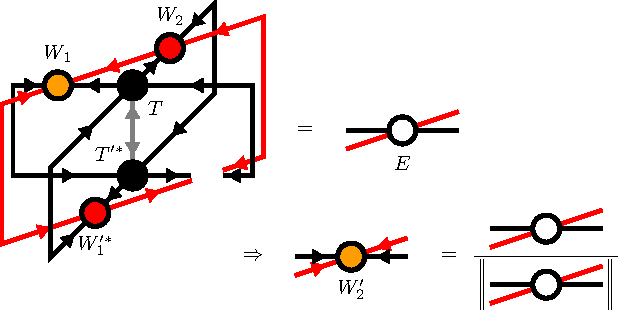
\includegraphics[scale=1]{figures/tikz/YB_isoTPS/yang_baxter_move_iterative/yang_baxter_move_iterative_d.pdf}
		\caption{}\label{fig:YB_move_iterate_polar_optimize_W2}
	\end{subfigure}%
	\caption{In this figure we show the three local updates that are used to iteratively solve optimization problem \eqref{eq:YB_isoTPS_YB_move_alternative_formulation}. (a) The tensor $T^\prime$ can be updated similarly by contracting all tensors except $T^\prime$ into the environment $E$ and isometrizing $E$ using an SVD. (b) The tensor $W_1^\prime$ can be updated by contracting all tensors except $W_1^\prime$ into the environment $E$, which is subsequently isometrized using an SVD. (c) To optimize the tensor $W_2^\prime$, all tensors except $W_2^\prime$ are contracted into the environment $E$. The updated tensor is then given as $W_2^\prime = E/\lVert E\rVert$.}
	\label{fig:YB_move_iterate_polar}
\end{figure}
The computational cost of the algorithm is dominated by the tensor contractions, scaling as $\mathcal{O}(3N_\text{iter}(\chi^2D^6d + \chi^3D^4)) = \mathcal{O}(N_\text{iter}D^8)$ for one YB move.\par
\begin{figure}
	\centering
	\begin{tikzpicture}[scale=1, trim axis left, trim axis right]
		\begin{axis}[xlabel=$N_\text{iters}$, ylabel={$\lVert|\Psi\rangle-|\Psi^\prime\rangle\rVert$}, grid=both, grid style={gray!20}, every axis plot/.append style={very thick}, scale only axis, height=\singleFigureHeight, width=\singleFigureWidth]
			
			\addplot[color = 5blue4]
			table[x=N_iter, y=trunc_error, col sep=space]{figures/plots/disoTPS/data/iterate_polar.txt};
			%\addlegendentry{Evenbly-Vidal}
			
		\end{axis}
	\end{tikzpicture}
	\caption{We show a cool figure here!!\todo{Caption}}
	\label{fig:disoTPS_tripartite_decomposition_iterate_polar}
\end{figure}
In practice we observe that the discussed algorithm converges only very slowly. To qualitatively showcase this, we perform the YB move on a typical environment of tensors $\left\{W_1, W_2, T\right\}$ that was encountered during imaginary time evolution of the Transverse Field Ising model, see Chapter \ref{chap:TFI} for more details. The bond dimensions chosen for the YB-isoTPS are $D = 4$, $\chi = 24$. We plot the error $\lVert\ket{\Psi}-\ket{\Psi^\prime}\rVert$ against the number of iterations in Figure \figref{fig:YB_isoTPS_tripartite_decomposition_iterate_polar}. After $N_\text{iter}=10000$ iterations, the algorithm is still not converged.

\subsection{Tripartite decompositon using an SVD and disentangling}
\label{sec:YB_move_svd_disentangle}
Alternatively, the constrained optimization problem \eqref{eq:disoTPS_YB_move_standard} can be solved via two successive SVDs with an optional disentangling prodcedure with the goal of reducing the truncation error or some entanglement measure. This is the same algorithm that was used for the MM in the original isoTPS \cite{cite:efficient_simulation_of_dynamics_in_two_dimensional_quantum_spin_systems}. The algorithm is sketched in figure \figref{} and is made up of three main steps.
\begin{enumerate}
	\item We start by contracting the tensors $T$, $W_1$ and $W_2$ into a single tensor $\Psi$ (figure \figref{} (b)). This tensor is then split from left to right via a truncated SVD
	\begin{equation}
		\Psi = XSZ^\dagger = X\left(SZ^\dagger\right) \eqqcolon X\theta
	\end{equation}
	as shown in figure \figref{}(c). The bond dimension is truncated to $D^2$.
	\item Next, we split the index of the bond connecting $X$ and $\theta$ into two indices of dimension $D$ each, see figure \figref{}(d). To proceed, we note that there exists a degree of freedom on the bonds connecting $X$ and $\theta$: A unitary $U$ and its adjoint can be inserted as shwon in figure \figref{}(e) without changing the result of the contraction
	\begin{equation}
		XU^\dagger U\theta = \left(XU^\dagger\right)\left(U\theta\right) \eqqcolon T^\prime \tilde{\theta}.
	\end{equation}
	This unitary $U$ can be chosen to minimize the truncation error of the next step by \textit{disentangling} the tensor $\theta$. We will discuss procedures of finding such a \textit{disentangling unitary} on the next page.
	\item In the last step, the tensor $\tilde{\theta}$ is split vertically into $W_1^\prime$ and $W_2^\prime$ using a truncated SVD as shown in figure \figref{}(f). Here, the bond dimension is truncated to $\chi$. We end up with the three tensors $T^\prime$, $W_1^\prime$ and $W_2^\prime$, completing the YB move.
\end{enumerate}
Before we discuss the disentangling procedure, two comments about step two of the above algorithm are in order. Firstly, there exists a degree of freedom for splitting the bond index, because applying the same permutations to the columns of $X$ and rows of $\theta$ does not change the result of contracting the network. Thus, there is no unique splitting that can be chosen. However, this degree of freedom is fixed by the disentangling process, making the exact permutation of the bond splitting irrelevant. Secondly, note that near the edges of the lattice it can happen that the matrizized tensor $\Psi$ has $\tilde{\chi} < D^2$ rows. In this case, the bond dimension after the SVD will also be $\tilde{\chi}$ and we cannot split the bond into two bonds of dimension $\chi_1=\chi_2=D$. Instead, we choose a splitting $\chi_1 \le D$, $\chi_2 \le D$ such that $\chi_1\cdot\chi_2$ is maximized while it must still hold $\chi_1\cdot\chi_2\le\tilde{\chi}$. We additionally prefer "equal" splittings $\chi_1\approx\chi_2\approx\sqrt{\tilde{\chi}}$ if possible. One can find such a splitting easily by computing all possible combinations of $\chi_1$ and $\chi_2$ and keeping only the best one. This has a computational cost of $\mathcal{O}\left(\sqrt{\tilde{\chi}}\right) = \mathcal{O}\left(d\right)$. \par
\begin{figure}
	%\includegraphics[width=0.8\textwidth]{figures/Tensor_Networks/yb_move_svd_disent.jpeg}
	\caption{test\todo{Why does this image not work? Also write caption.}}
	\label{fig:yb_move_svd_disent}
\end{figure}
We will now discuss the problem of finding a good disentangling unitary $U$ for step two of the above algorithm, which is crucial for the performance of the YB move. The problem can be formulated as follows: Given a tensor $\theta \in \mathbb{C}^{\chi_1\times d_1\times d_2\times \chi_2}$, find a unitary $U\in\mathbb{C}^{d_1\times d_2\times d_1\times d_2}$ minimizing a cost function
\begin{equation}
	f(\tilde{\theta}),
\end{equation}
where
\begin{equation}
	\tilde{\theta}\in\mathbb{C}^{\chi_1\times d_1\times d_2\times \chi_2}, \quad \tilde{\theta}_{\alpha,i,j,\beta} \coloneqq \sum_{i^\prime,j^\prime}U_{i,j,i^\prime,j^\prime}\theta_{\alpha,i,j,\beta}.
\end{equation}

\subsection{Comparison of the two algorithms}
\label{sec:YB_move_comparison}
\todo{TODO!}